\label{key}\documentclass[letterpaper, 12pt,oneside]{article}
\usepackage{amsmath}
\usepackage{graphicx}
\usepackage{xcolor}
\graphicspath{{Imagenes/}}
\usepackage[utf8]{inputenc}
\usepackage{listings}
\usepackage[hidelinks]{hyperref}

\title{\Huge Taller de Herramientas Computacionales}
\author{Josué Artemio Hernández Rodríguez}
\date{24/Enero/2019}

\begin{document}
	\maketitle
	\begin{center}
		
\includegraphics[scale=0.7]{3.jpg}
	\end{center}

	\newpage
	
	\title{\huge \textit{Bitácora problema 9 }}\\

	Este problema pide al usuario una palabra, y te la regresa pero invertida. Para poder hacer esto, primero se inicia con una variable que contiene una cadena vacía, el contador que es la longitud de la cadena len(cadena) y una variable indice = -1. Se inicia el bucle con while con la condición contador >= 1: que la variable invertida sea igual a la suma de cadena[indice] y luego el indice cambia a ser "indice - 1" y el contador va disminuyendo en -1 
	
	
	
	
	
	
	  
	 

	\begin{figure}[h]
		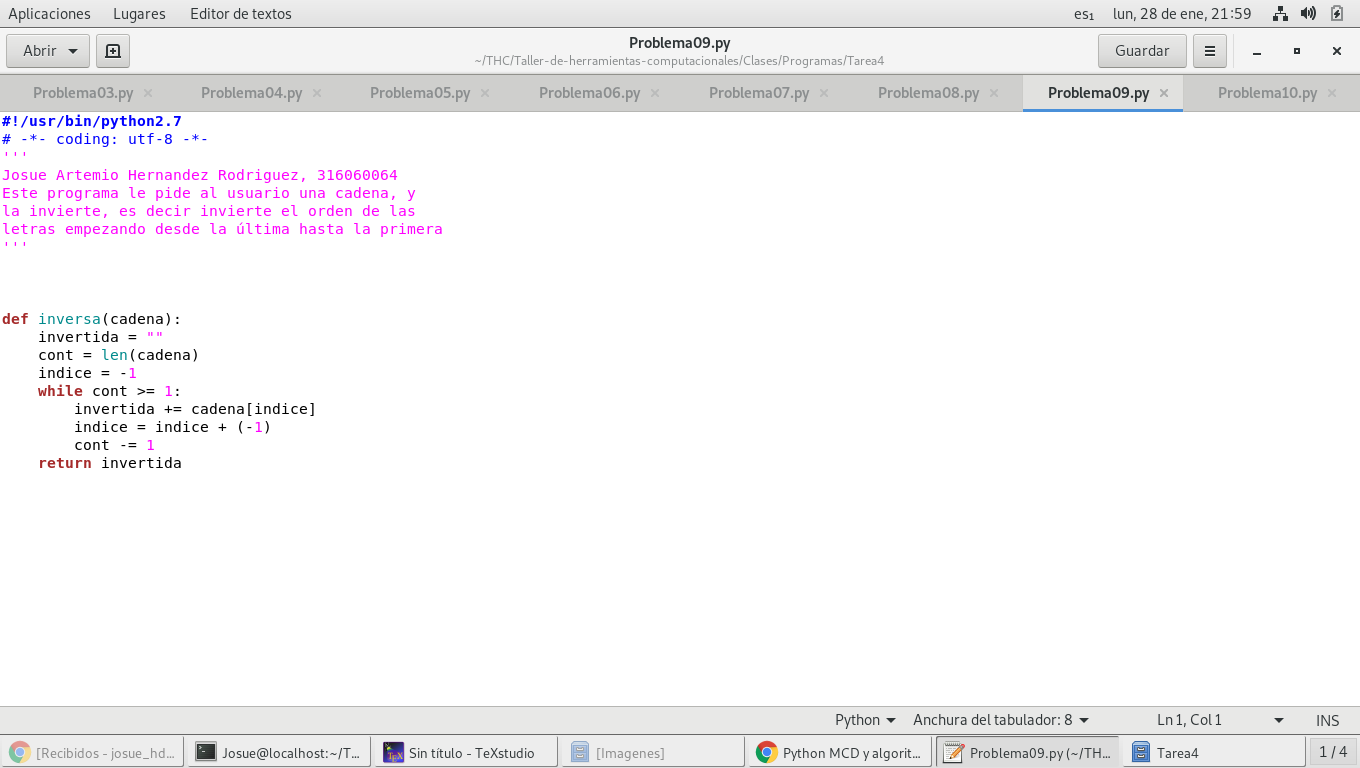
\includegraphics[scale=0.4]{pro09.png}
		
	\end{figure}

	
	
\end{document}
